\chapter{Systematic Trading Rules}
\bichaptertitle{系统化交易规则}

\noindent\textsc{A trading rule is a systematic way of predicting price movements.} Trading
rules are a core component of any trading system, so how can you find trading rules that
will work? Why do they work? What styles of trading are available? Finally, how
successful should you expect trading rules to be?

\noindent\textsc{交易规则是一种以系统化方式预测价格变动的方法。}
交易规则是一切交易系统的核心组成部分，
那么究竟该如何找到真正有效的交易规则？
它们为什么会有效？
市场上又有哪些不同的交易风格？
最后，
对于交易规则的成功程度，
你又应该抱有什么样的现实预期？

\section*{Chapter overview}
\phantomsection
\addcontentsline{toc}{section}{Chapter overview}
\bisectiontitle{本章概览}

\begin{tabularx}{\textwidth}{@{}p{0.28\textwidth}Y@{}}
\textbf{What makes a good trading rule} & Some key elements that make a trading rule more
likely to be successful. \\
\textbf{When trading rules don't work} & Reasons why a trading rule which worked in
back-test may not work in practice when actually traded. \\
\textbf{Why are certain rules profitable?} & Explanations for why profit making rules exist,
to help you work out if that profitability is likely to be repeatable. \\
\textbf{Classifying trading styles} & The main ways in which you can classify rules into
trading styles, and the important characteristics each style has. \\
\textbf{Achievable Sharpe ratios} & What are realistic Sharpe ratios to expect? \\
\end{tabularx}

\medskip

\begin{tabularx}{\textwidth}{@{}p{0.28\textwidth}Y@{}}
\textbf{什么样的交易规则才算好} & 那些让交易规则更可能成功的关键要素。 \\
\textbf{交易规则什么时候会失效} & 为什么一条在回测中有效的规则，到了真实交易里可能就失灵。 \\
\textbf{为什么某些规则会盈利} & 对“赚钱规则为何存在”的解释，从而帮助你判断这种盈利是否可重复。 \\
\textbf{如何给交易风格分类} & 将规则划分到不同交易风格的主要方式，以及各风格的重要特征。 \\
\textbf{可实现的 Sharpe 比率} & 你应当对 Sharpe 比率抱有什么样的现实预期。 \\
\end{tabularx}

\section*{What makes a good trading rule}
\phantomsection
\addcontentsline{toc}{section}{What makes a good trading rule}
\bisectiontitle{什么样的交易规则才算好}

\audiencebox{Staunch systems trader}{This section mostly relates to how trading rules are
fitted. This is less applicable to asset allocating investors and semi-automatic traders, and
they can skip to ``Why are certain rules profitable?''\par\medskip
坚定的系统化交易者\par\medskip
这一节主要讨论交易规则是如何被拟合出来的。
它对资产配置型投资者和半自动交易者的相关性较弱，
他们可以直接跳到
“为什么某些规则会盈利？”}

\subsection*{It is carefully built from ideas or data}
\bisubsectiontitle{它应当是从想法或数据中被谨慎构建出来的}

Systematic trading assumes the future will be like the past. Hence you should create rules
that would have worked historically, and hope that they will continue to work.

But there are at least two different ways to find rules that made money in the past. One
common method, which I call data first, is to analyse some data, find some profitable
patterns and create some trading rules to exploit them. This is sometimes called data
mining. The alternative, ideas first, is to come up with an idea, then create a rule, which
is then tested on data to see if it works.\footnote{There is a third method which is to use an
idea which you cannot or will not test on historical data. Strictly speaking, this wouldn't
be systematic trading.\par 还有第三种方法：你直接使用一个自己既不能也不愿意在历史数据上测试的想法。
严格说来，那已经不属于系统化交易了。}

\begin{quote}
``There's a creative moment when you think of a hypothesis, maybe it's that interest rate
data derives currency rates. So we think about that first before mining the data. We don't
mine the data to come up with ideas.''
\end{quote}

\begin{quote}
“当你想到一个假设时，会有一个创造性的瞬间。比如，你可能想到利率数据会驱动汇率。
所以我们会先从这个想法出发，然后才去挖掘数据。我们不会通过挖掘数据来生成想法。”
\end{quote}

\noindent\begin{center}
  \begin{tabularx}{\textwidth}{@{}Y Y@{}}
    \toprule
    \textbf{Advantages of ideas first} & \textbf{Advantages of data first} \\
    \midrule
    If an idea works no further potentially dangerous fitting is required. &
    There will be a bias with ideas first to testing things that you know will work,
    either because of ``market lore'' or academic studies. This is a form of implicit
    over-fitting. \\
    Any fitting will probably be done in a small subset of alternatives. &
    With ideas first it is tempting to try a large number of ideas to find the ones that
    work. This is definitely over-fitting. \\
    You tend to get simpler and more intuitive trading rules with ideas first. &
    In data first all the fitting is explicit, so the degree of over-fitting can be controlled. \\
    You can construct rules that make intuitive sense, with a story behind them. &
    A compelling theory or story does not guarantee that the source of returns is
    repeatable, and could give a false sense of security. This is the narrative fallacy I
    mentioned in Chapter 1. \\
    It's easier to classify the trading rule and work out where its profits are coming from. &
    Clever data analysis might unearth novel strategies that were previously unknown. \\
    \bottomrule
  \end{tabularx}
\end{center}

\medskip

\noindent\begin{center}
  \begin{tabularx}{\textwidth}{@{}Y Y@{}}
    \toprule
    \textbf{“想法优先”的优势} & \textbf{“数据优先”的优势} \\
    \midrule
    如果一个想法成立，就不需要再做额外、且可能很危险的拟合。 &
    “想法优先”会有一种偏差：你更容易去测试那些你原本就知道可能有效的东西，
    无论这种判断来自“市场经验之谈”还是学术研究。这是一种隐性的过拟合。 \\
    任何拟合往往也只会发生在一小部分备选方案内部。 &
    在“想法优先”中，你很容易忍不住尝试大量想法，去找出那些真正有效的。
    这无疑属于过拟合。 \\
    “想法优先”通常会产生更简单、更直观的交易规则。 &
    在“数据优先”中，所有拟合都是显式进行的，因此过拟合的程度反而更容易被控制。 \\
    你可以构建出那些在直觉上讲得通、背后也有明确故事的规则。 &
    一个很有说服力的理论或故事，并不能保证这种收益来源真能重复出现，
    反而可能制造虚假的安全感。这就是我在第一章提到的叙事谬误。 \\
    你更容易给交易规则分类，也更容易理解利润到底来自哪里。 &
    聪明的数据分析可能会挖掘出此前无人知道的新策略。 \\
    \bottomrule
  \end{tabularx}
\end{center}

设计一套“想法优先”的系统，就像是在说：“我想设计一套能够捕捉这种收益来源的系统。
我希望这种收益来源在未来仍然存在。”

而“数据优先”的系统则更像是在说：“这里有一套过去能够赚钱的系统，
它利用的是市场中曾经出现过的某种模式
（至于这种模式为什么存在，我既不打算解释，也不打算理解）。
我希望这些模式在未来继续存在。”

根据我的经验，真正能够长期持续赚钱的交易，通常来自谨慎的研究，
而研究者本身既有知识，也会认真思考自己的利润到底来自哪里。
我见过那些最后赔钱的系统化交易，
很多往往都是随意挖掘数据的结果；
做这种挖掘的人，
既不去考虑为什么某条规则过去看起来赚钱，
也不去考虑它未来为什么可能不再赚钱。

正因为有这些经验，再加上我个人更偏好那些我能够信任、也能够理解的东西，
所以我总体上更偏向“想法优先”的方法。
这种方法通常会产生更直观、更简单、也更透明的规则。
只要你测试的想法数量不多，过拟合出现的概率也会更低。
在下一章“拟合”里，我重点讨论的也是“想法优先”的测试方式，
因为它更简单，而且不需要太复杂的技巧就能相对安全地实施。

当然，在某些情形下，“数据优先”也可能更好。
例如在高频交易中，数据量很大，规则可以被定期重新拟合，
而且随着市场结构不断演变，也更可能发现新的想法。

你应当了解自己偏好方法的长处和短处，
并在合适的地方使用它。

系统化交易默认未来会在某种程度上像过去，因此你会想去构建那些“在历史上有效”的规则，并寄望它们在未来仍然有效。
而找到这种规则，至少有两条路。第一条是“数据优先”：先分析数据，找出历史上赚钱的模式，再针对这些模式写出规则，这往往会滑向数据挖掘。
第二条是“想法优先”：先形成一个关于市场为何会给你回报的想法，再把它写成规则，并用数据去验证。

就我自己的经验来看，长期持续赚钱的系统，大多来自深思熟虑、真正理解收益来源的人所做的研究；
而那些最后赔钱的系统，很多都是随意挖掘数据、
却根本不去思考“它过去为何赚钱、未来为何可能不赚钱”的产物。
因此，
我总体上更偏好“想法优先”：
它往往能产生更直觉、更简单、更透明的规则，
也更容易被信任和理解。
当然，
在像高频交易这类拥有大量数据、
且市场结构持续变化的领域里，
“数据优先”也可能更有优势。

\subsection*{Explainable profits}
\bisubsectiontitle{利润应当是可解释的}

理解交易规则为什么会赚钱非常重要。如果你知道某件事过去为什么能盈利，
那你也就能大致判断这种利润是否还会延续，
或者这条规则会在什么时候、又因为什么而失效。

在“想法优先”的路径下，
你通常很容易解释一条策略为什么盈利，
因为解释本来就包含在最初的想法里。
例如，你也许测试了一条趋势跟随规则，
而你认为它之所以赚钱，
是因为前景理论所描述的那些认知偏差。

而在“数据优先”的路径下，
任何解释都只能在拟合完成之后再去补。
你得先观察一条规则是如何表现的，
然后再反推出可能是什么机制造成了这种效果。
一条数据驱动规则越复杂，
你就越难把它解释清楚。

不过，寻找解释本身也有风险。别忘了叙事谬误，
这同样是一种认知偏差：人类喜欢故事。
哪怕一条规则在统计检验下站不住脚，
只要它拥有一个足够有说服力的解释，
我们就更容易相信它。
就我自己而言，
想要真正信任一条交易规则，
我既希望它有一个好故事，
也希望它有一个严格的回测。

\subsection*{Intuitively understandable behaviour}
\bisubsectiontitle{行为应该在直觉上可理解}

一个在直觉上说得通的策略，会更容易被信任。
如果你在联合利华发布财报前，
看到它的股价正在上涨，
那么一套趋势跟随系统理应正在买入。
如果这套策略反而在卖出，
那就值得警惕，
你也许会去检查是不是数据有误，
或者软件里藏着 bug。
而在大多数情况下，
你看到的行为都会符合预期，
于是你就能放心下来。

一套复杂系统则可能会在价格上涨时买入，
也可能在价格上涨时卖出，
这完全取决于背后的具体模式。
这样一来，
它的行为就会显得没那么明显，
也更难预测。

\subsection*{As simple as possible}
\bisubsectiontitle{尽可能简单}

解释简单交易规则的盈利来源和行为模式，要容易得多。
这类规则通常只有很少几个部件，
也不存在奇怪的交互作用。
“想法优先”的规则本来就应该保持简单，
除非你一开始的想法就异常复杂，
或者你为了让回测更赚钱而故意把它做得越来越复杂；
而这两种做法我都不推荐。

“数据优先”的规则可以非常简单，
也可以极其复杂，
这取决于你拟合了多少参数。
参数越多的数据优先规则，
就越难解释，
也越容易遭受过拟合。
不过，
一条复杂的数据优先规则，
也可能捕捉到那些更简单规则看不到的新型交易模式。

\subsection*{Can be systematised}
\bisubsectiontitle{必须能够被系统化}

任何想法最终都必须被翻译成系统化规则。并不是所有交易风格都适合这样做，
因为有些方法天生过于主观，另一些则会受到数据限制。
不过，即便如此，它们仍然可以像我在半自动交易者示例中展示的那样，
被包裹进一套系统化的仓位管理框架之中。

\subsection*{Too subjective}
\bisubsectiontitle{太主观}

许多交易方法之所以无法系统化，是因为你根本不可能把它们写成一组相对简单、客观而通用的规则。
例如，对于一些更玄奥的技术分析流派，
要把某个名字古怪的 K 线形态精确转换成规则就很困难。
另一个例子是并购套利：
你必须根据许多很难量化的因素去判断一笔交易最终能否完成。

\subsection*{Data limitations}
\bisubsectiontitle{数据限制}

即便一条策略本身是客观的，所需数据也可能根本拿不到。
就算你真的能为并购套利写出交易规则，
涉及法律与监管问题的那些必要信息，
也很难被转换成一种适合算法处理的格式。

还可能存在数据量不足的问题。
正如你会在下一章“拟合”里看到的，
要真正检验一条策略，往往需要很多年的数据。
近来有些对冲基金会使用 Google 搜索热度、Twitter 趋势之类的数据来预测市场。
这些想法很适合写成新闻稿，
但要想严肃评估它们，
未来很多年里都还拿不到足够的数据。

你还可能会在不同品种之间的数据可比性上遇到困难。
例如，会计指标在不同国家之间并不一致，
因为相关规则和标准并不相同。
这就让跨国股票价值策略变得难以实施。

好的规则不仅要“理论上成立”，还要能够被清晰地写成客观规则，并且拥有足够、可比且可获得的数据。
很多看似聪明的交易方法之所以无法系统化，不是因为想法不有趣，而是因为它们太主观，或根本没有足够的数据来支撑。

\section*{When trading rules don't work}
\phantomsection
\addcontentsline{toc}{section}{When trading rules don't work}
\bisectiontitle{交易规则何时会失灵}

\audiencebox{Staunch systems trader}{This section mostly relates to how trading rules are
fitted. This is less applicable to asset allocating investors and semi-automatic traders. They
can skip to ``Why are certain rules profitable?''\par\medskip
坚定的系统化交易者\par\medskip
这一节主要和交易规则拟合有关。
对资产配置型投资者和半自动交易者的相关性较弱，
他们可以直接跳到
“为什么某些规则会盈利？”}

一条在回测中表现成功的规则，在现实里可能失败，原因有很多。

\subsection*{It never really worked}
\bisubsectiontitle{它其实从来就没真正有效过}

第一种情况是：有些规则在回测中看起来有效，
但如果放回历史现场，其实根本赚不到钱。
这些规则可能是过拟合的，
我会在下一章详细讨论这一点。
另一种可能是，
它们依赖的是前视数据，
而这些数据在现实中发布会有延迟，
但在回测里却被错误地当作即时可得。
你所考虑的品种中也可能存在幸存者偏差。
你还可能低估了交易成本，
或者漏掉了当时市场结构中的某个关键因素，
例如股票卖空约束。
最后，你所使用的历史样本也可能太短，
从而错过了一个至关重要的时期：
在那里，这条策略本来会彻底炸掉。

\subsection*{The world changes}
\bisubsectiontitle{世界会变化}

你想要的是那些过去有效、而未来也能继续有效的策略。
但如果你试图利用的那种行为模式或者市场结构本身消失了呢？

例如，如果一大群系统化交易者都在使用同样的规则，并开始主导某个市场，会发生什么？
相关策略难道不会全部失效吗？
这个问题对相对价值策略尤其严重，
因为这类策略本来就是在资产变便宜时买入、变昂贵时卖出。
一旦市场里存在大量相似系统，
任何轻微错价都会被立刻修正，
于是收益也会消失。

相反，趋势跟随者在集体主导市场时，
也许会乐于看到趋势被进一步强化；
但一旦价格反转，
他们也可能被卷入一场同步发生的逃命式离场。

在那些计算机拥有显著优势的领域，
例如超高频交易，
人类几乎已经被彻底挤出。
这些策略不再是在利用人类弱点或市场结构，
而是在一场纯粹靠速度和预判对手反应来取胜的军备竞赛中厮杀。
这一领域完全不属于本书讨论的范围。

一条规则即便在过去有效，也可能因为根本从来没真正有效过、因为使用了前视信息、因为忽略了幸存者偏差、
因为低估了成本，或者因为它恰好躲过了最致命的历史时期而显得“很好看”。
此外，市场本身也会变化。一个曾经存在的行为模式可能会消失；一种原本有利可图的错价修复机制，
可能会因为太多人采用同样的策略而被迅速抹平。

\section*{Why certain rules are profitable}
\phantomsection
\addcontentsline{toc}{section}{Why certain rules are profitable}
\bisectiontitle{为什么某些规则会盈利}

\audiencebox{This section is relevant to all readers}{Whether you are using systematic rules
or making discretionary forecasts it's important to understand where your returns are
coming from and what your ``edge'' is --- if any. This section briefly covers the theory
around this subject.\footnote{An exhaustive treatment of this topic can be found in
\textit{Expected Returns} by Antti Ilmanen.\par 关于这一主题的系统性论述，
可以参见 Antti Ilmanen 的
\textit{Expected Returns}。}
It presents some possible reasons why certain
assets, portfolios of assets, or dynamic trading rules make profits.\par\medskip
本节与所有读者相关。
无论你使用的是系统化规则还是主观预测，
理解收益到底来自哪里、
自己的“边”
（如果有的话）究竟是什么，都非常重要。
这一节会简要介绍相关理论，
并给出一些可能的理由，
说明为什么某些资产、
资产组合或动态交易规则能够盈利。}

\subsection*{Risk premia}
\bisubsectiontitle{风险溢价}

当你购买保险时，你要支付保费。
保费的定价水平会使保险公司预期自己虽然偶尔会遇到大额赔付，
但长期平均下来仍然能够盈利。
保险购买者从长期看注定是亏钱的，
但作为交换，
他们获得了对罕见重大损失的保障。
金融市场里也存在这两种不同的收益形态，
所以“买保险”和“卖保险”的类比非常有用。

任何愿意购买“金融保险”的人，
都会甘愿承受低于平均市场收益的回报；
而那些愿意出售这类保险的人，
则会因为赚取风险溢价而获得更高收益，
这就类似于保险公司的利润。
某些资产对某类风险暴露得更多；
买入这些资产，就会带来来自各种风险溢价的额外收益。

\subsection*{Persistent risk premium}
\bisubsectiontitle{持续性的风险溢价}

有些风险溢价会持续很长时间，
比如投资股票而不是债券这类更安全资产时，
你通常会期待得到额外回报。
在股票价值策略中，
还有许多其他风险因子，
例如账面市值比和公司规模。
在其他资产中，
也存在不同形式的溢价。
例如，期限更长的债券通常会比更早到期的债券赚取更高溢价，
因为投资者希望在出借期限更长时获得额外补偿。

\subsection*{Timing varying risk premium}
\bisubsectiontitle{随时间变化的风险溢价}

如果你在 2006 年买入针对高风险抵押贷款的廉价 CDS 保险，
那么当一年后市场崩塌时，
你就会像对冲基金经理 John Paulson 那样赚到数十亿美元。
反过来，
当市场“街头血流成河”时，
你也可能以极低价格买到高风险资产，
就像 2009 年初我买入巴克莱时那样，
只是我当时买得还不够激进。

显然，风险溢价并不是常数。
人们对风险的偏好会随时间变化，
在 2006 年那样相对亢奋的时期与 2009 年那样的恐慌时期之间来回摆动。
于是，你可以通过买入便宜的溢价、卖出昂贵的溢价来获利。
这其实是一种均值回归交易：
你假设溢价
--- 从而价格
--- 会回到某种长期均衡。

在实践中，
你几乎不可能准确地说出某项溢价的“正确”价值到底是多少，
并据此断定现在应该买入还是卖出。
市场也可能在很长时间里偏离这个正确值。
尽管如此，
这仍然是另一个非常有用的收益来源。

\subsection*{Skew and unlikely events premium}
\bisubsectiontitle{偏度与小概率事件溢价}

经典金融理论中的理性投资者，只关心一项资产的 Sharpe 比率
（SR）
--- 也就是用标准差调整后的平均收益。
只有当所有资产的收益分布都是对称的，
这种说法才真正成立。
但在现实中，
两个拥有相同 SR 的资产，
可能一个表现为持续小亏、偶尔大赚
（像买保险的人），
另一个则表现为持续小赚、偶尔大亏
（像卖保险的人）。
这意味着，
不同资产的收益偏度并不相同。

\subsection*{CONCEPT: SHARPE RATIO (SR)}
\bisubsectiontitle{概念：Sharpe 比率（SR）}

Sharpe 比率
（SR）
衡量的是一套交易策略或一项资产在过去有多赚钱，
或者预期会有多赚钱。
计算方法是：先看收益，
再按其风险进行调整。

严格来说，
你应当使用高于无风险利率的“超额收益”，
不过对使用衍生品的交易者来说，
这一点并不那么相关；
而在 2009 年之后的低利率时代，
它的重要性也比之前低得多。

形式化地说，
SR 就是某一时间周期内的平均收益，
除以同一周期内收益的标准差。
因此，日 SR 就是平均日收益除以日收益标准差。
不过我通常使用年化 Sharpe 比率
--- 也就是年化收益除以年化标准差。
如果一年有 256 个交易日，
那么年化 SR 大约是日 SR 的 16 倍。

Sharpe 比率并不是完美的指标。
尤其是，
它默认收益与亏损是对称分布的，
而这在现实中并不成立。
当你要比较的是“一种资产偶尔会出现巨大亏损”，
而另一种资产“偶尔会出现巨大盈利”时，
Sharpe 比率就没什么用了；
这时你必须把偏度考虑进来。

Sharpe 比率衡量的是“风险调整后的收益”。形式上，它等于某一时期内的平均收益除以同一时期内收益的标准差。
在本书中，我通常使用年化 Sharpe。它非常有用，但也并不完美，尤其是在面对明显非对称收益分布时。

\subsection*{CONCEPT: SKEW}
\bisubsectiontitle{概念：偏度}

在第一章讨论标准差时我说过，
对于对称的高斯正态分布来说，
大幅亏损出现的概率与大幅盈利相同。
例如，价格向上移动两个标准差，
出现概率大约是 2.5\%；
向下移动两个标准差，
概率也同样是 2.5\%。

但许多资产并不具备对称分布
--- 它们的收益会向某一侧倾斜。
在很多情况下，
大亏出现的概率会高于同等幅度的大赚。
例如，全球股市在 1987 年 10 月曾经单日下跌 20\%
--- 这大约是 20 个标准差
--- 但它们从未以同样速度单日暴涨过。

如果一项资产发生大幅下跌的概率，
高于发生同等幅度上涨的概率，
那它就被称为负偏度；
如果大幅上涨更可能，
那它就具有正偏度。

假设两项资产拥有相同的 Sharpe 比率，
那么正偏度资产的收益路径，
通常会包含更多亏损日，
但这些亏损日的损失都比较小；
而负偏度资产的下跌日会更少，
可是一旦下跌，损失往往更大。

回到前面那个类比，
买保险就是一种正偏度策略。
你会频繁地承受小亏损
（支付保费），
偶尔获得大收益
（拿到赔付）。
如果你是卖保险的人，
那就会频繁获得小收益，
但偶尔遭遇大亏损
--- 这就是负偏度。

图 5 和表 1 展示了两种偏度不同、
但 Sharpe 比率相同的资产，
它们的收益分布和统计特征会是什么样。

\begin{figure}[htbp]
  \centering
  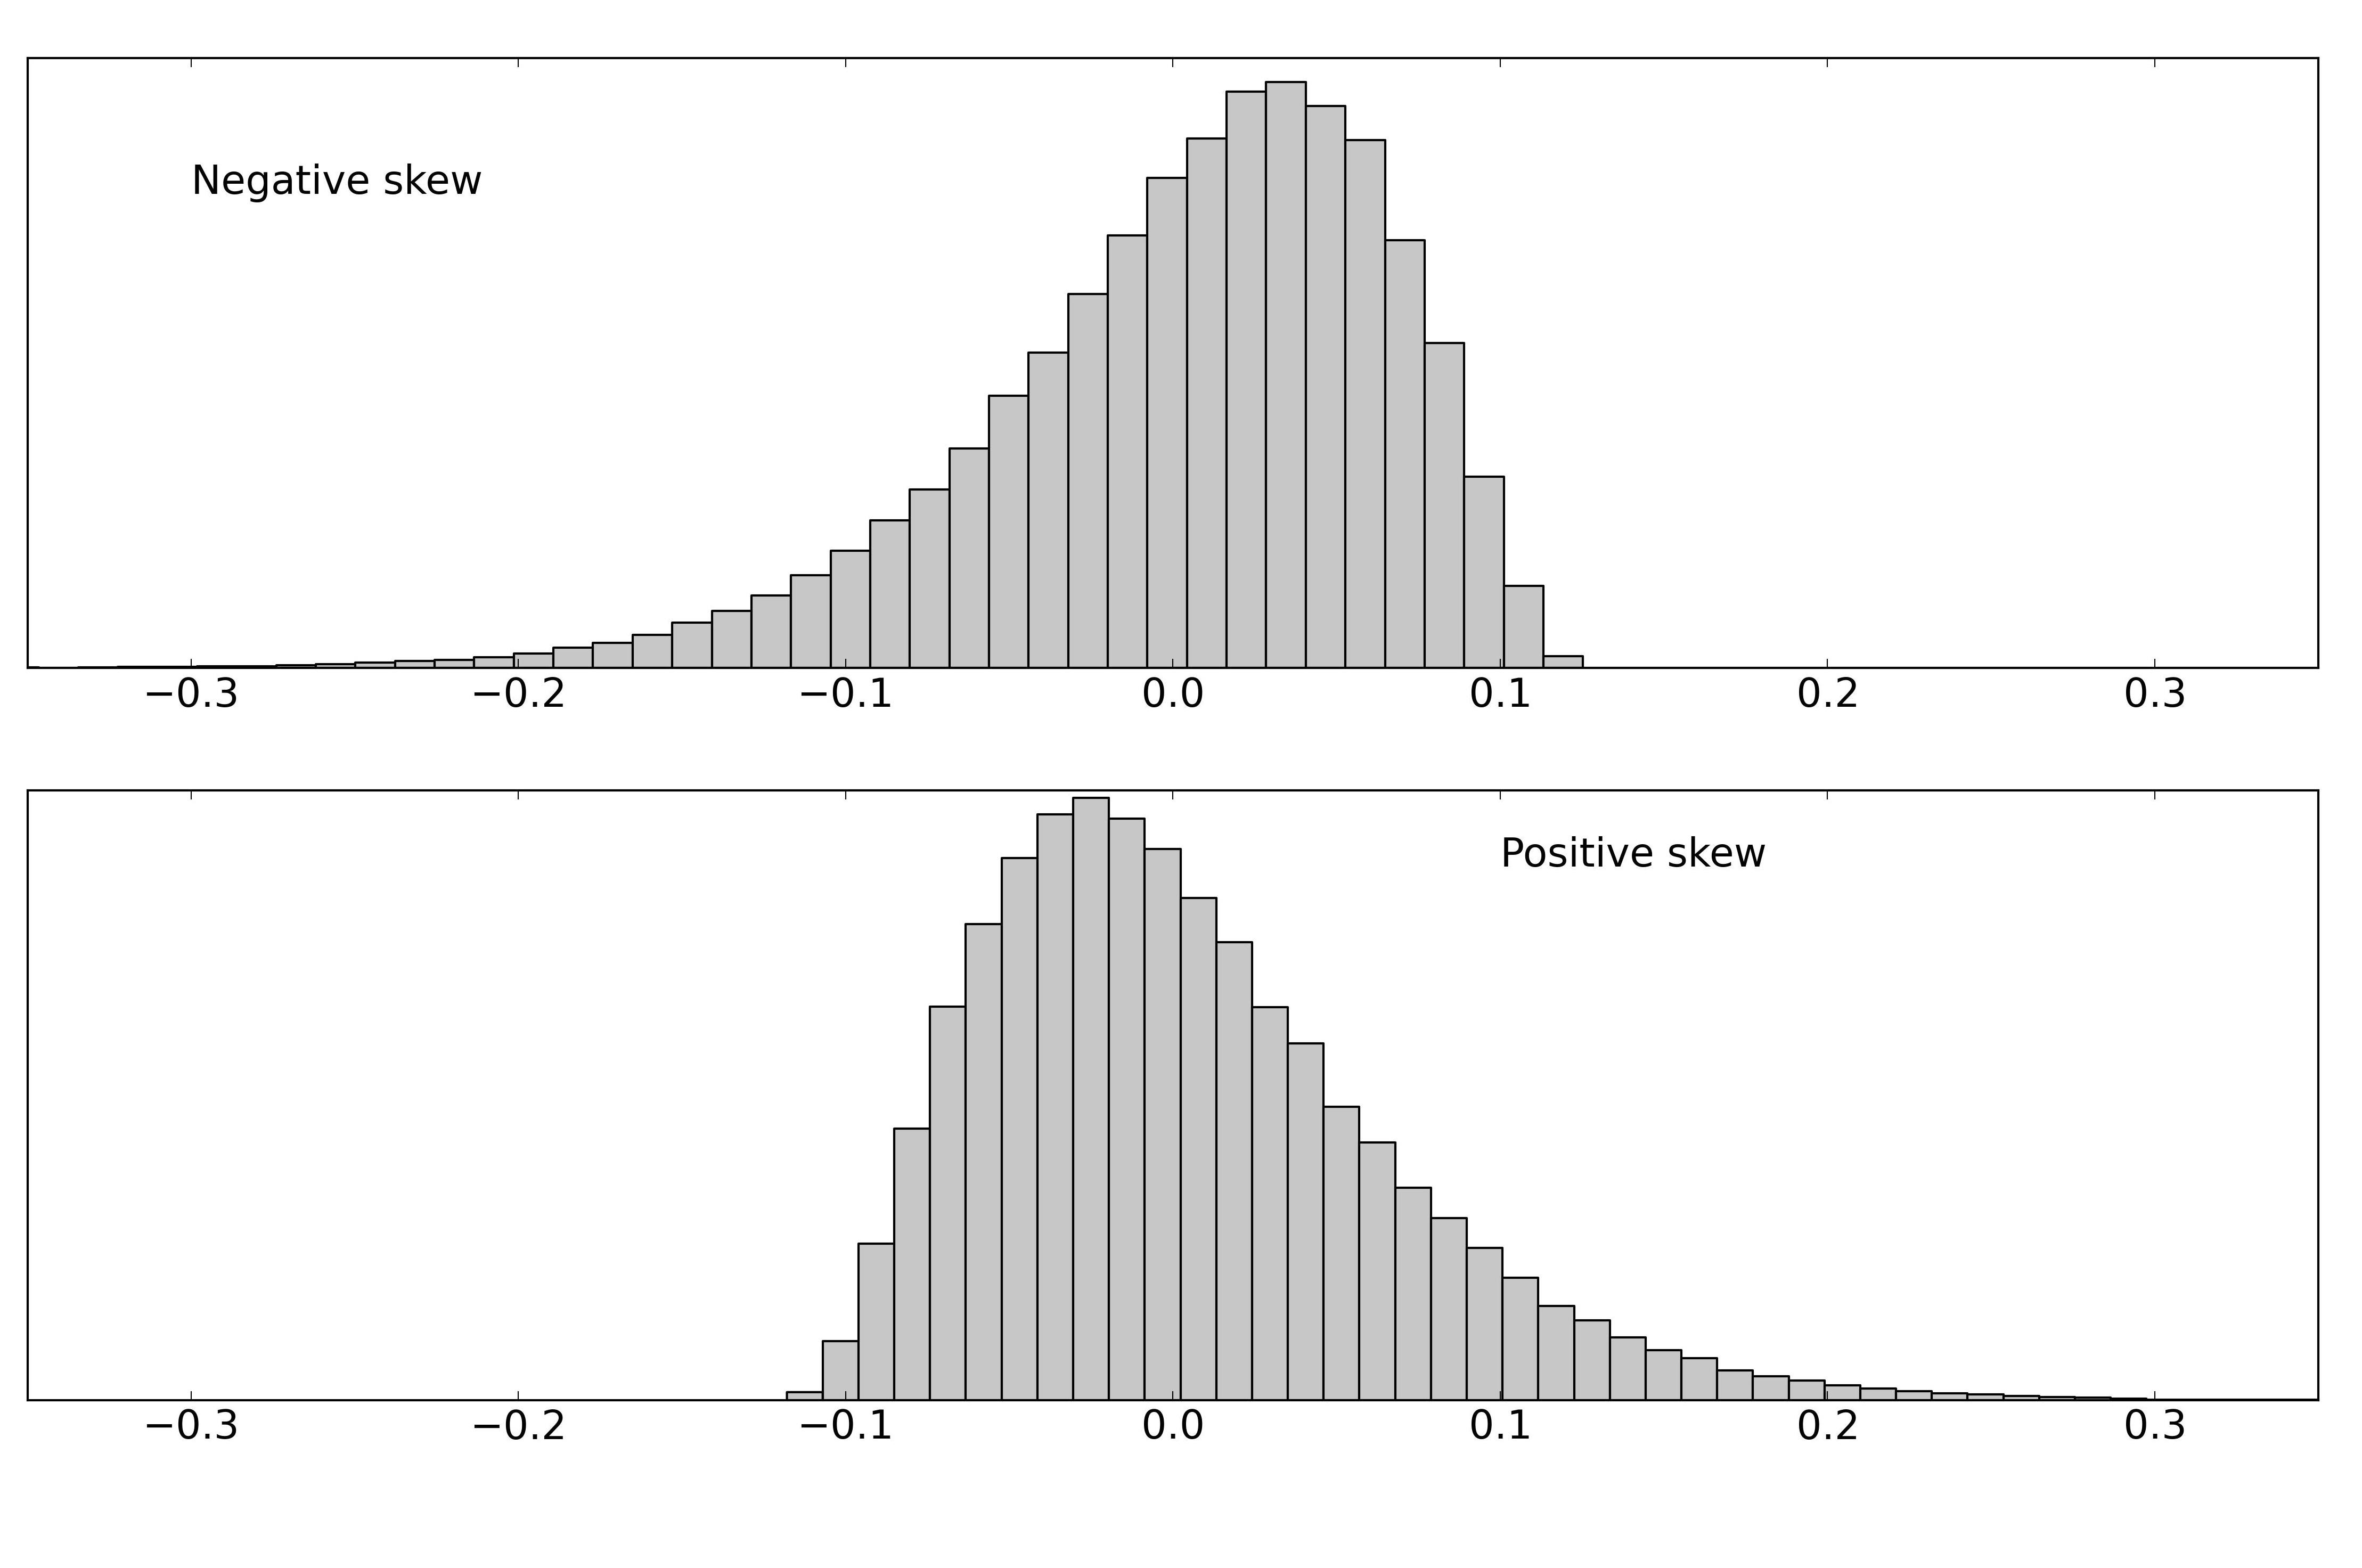
\includegraphics[width=\textwidth]{figures/raw/img-005.png}
  \caption{Two assets, same Sharpe ratio, different skews.\\
  两个资产：相同 Sharpe 比率，不同偏度。}
\end{figure}

\begin{table}[htbp]
  \centering
  \caption{Characteristics of negative versus positive skew\\
  负偏度与正偏度的特征比较}
  \begin{tabular}{@{}lcc@{}}
    \toprule
    & \textbf{Negative skew} & \textbf{Positive skew} \\
    \midrule
    Mean of daily returns & 0.4\% & 0.4\% \\
    Sigma of daily returns & 6.3\% & 6.3\% \\
    Annualised Sharpe ratio & 1.0 & 1.0 \\
    Skew of daily returns & -1.0 & 1.0 \\
    Median daily return & 1.4\% & -0.6\% \\
    Average Gain:Average Loss & 0.8 & 1.4 \\
    Hit rate (\% of positive returns) & 59\% & 46\% \\
    Expected annual worst daily loss & -22\% & -10\% \\
    Expected annual best daily gain & 10\% & 22\% \\
    \bottomrule
  \end{tabular}
\end{table}

偏度描述的是收益分布有多不对称。正偏度意味着多数时候是小亏，偶尔会有大赚；负偏度则意味着多数时候是小赚，偶尔会遭遇大亏。
同样的 Sharpe 比率，可能对应完全不同的“赚钱体验”与风险体验。比如买保险是典型正偏度，卖保险则是典型负偏度。

\subsection*{Leverage}
\bisubsectiontitle{杠杆}

你会借钱来投资吗？经典金融理论假设人们会自由地借钱，
但现实中许多投资者既做不到，也不愿这么做。
对业余交易者而言，
借保证金买股票依然不是常见行为。
虽然期货、差价合约等衍生品的可得性已经大幅提高，
它们仍然主要是少数勇敢者的工具。
很多机构基金同样不使用借贷，
而另一些即便愿意使用，
也会受到监管者和经纪商施加的限制。

这意味着，
那些 Sharpe 比率很高、
但绝对收益较低、
同时波动率更低的资产，
仍然不会受到那些追求高收益、
又无法借钱加杠杆的投资者欢迎。
他们宁愿去买那些绝对收益更高、
但风险也更大的资产，
即便新增风险并没有被完全补偿，
即便它们的 SR 反而更低。

于是，
缺乏分散化的投资组合就会很常见，
比如几乎全部波动率都来自股票。
人们偏好风险更高的股票，
1999 年的科技泡沫就是一个极端例子。
这一效应也解释了为什么：
历史上短久期债券的 SR 往往高于长久期债券。
那些幸运到能够合理使用杠杆的投资者，
从长期看理应优于其他人。
但一定要小心：
一旦危机来临，
建立在债务之上的投资组合很容易陷入死亡螺旋。
价格下跌，
经纪商要求补保证金或者干脆收紧借贷，
投资者被迫卖出，
而价格又继续下跌。
这种在最糟糕价格点发生的被迫抛售，
足以抹掉多年的利润。

我会在第九章“波动率目标”中进一步讨论如何安全地使用杠杆。

\subsection*{Liquidity and size}
\bisubsectiontitle{流动性与规模}

一项资产的流动性，
指的是我们能够在不过度影响价格的前提下，
多容易买入或卖出它。
大型机构投资者往往必须以大规模买入，
并在客户赎回时迅速平仓，
所以他们偏好高流动性资产。
于是，相对于那些流动性较差的替代品，
高流动性资产的价格会被推高。
这也就解释了一个众所周知的现象：
小公司往往能提供更高回报。
流动性溢价同样解释了土地、风险投资等“另类”资产为何有吸引力。
那些愿意长期持有低流动性组合的投资者，
也就拥有更大的机会获得更高收益。

流动性、规模与杠杆所对应的溢价还会随时间变化，
从而创造出择时买卖的机会。
例如，
在 2006 年底，
与抵押贷款支持资产相关的衍生品仍然流动充足，
因此价格带有溢价；
但一年之后，
它们几乎已经难以交易，
愿意接盘的人甚至可以在严重下调后的官方报价基础上，
再拿到相当可观的折扣。

\subsection*{When others have to trade}
\bisubsectiontitle{当别人被迫交易时}

并不是所有人交易都是为了赚钱。
有些人是被迫交易。
例如，
那些希望维持本币弱势的央行
--- 比如瑞士或日本
--- 如果愿意承担相应成本，
理论上就可以无限期地这么做。

于是，一条外汇 carry 规则如果在瑞士这类低利率货币中融资，
再投资到高利率货币中，
就会因此持续盈利，
至少在这种汇率政策被放弃之前都如此
（瑞士在 2015 年 1 月就放弃了相关政策）。
但这类策略也会带来突如其来的巨大亏损，
因此 carry 是一种非常典型的负偏度策略。

其他资产类别里也有类似例子。
例如，
为了减少税负或者“粉饰”资产负债表而进行的年末交易，
会在股票价格中制造季节性效应。
保险公司可能不得不买入稀缺的长久期债券来对冲负债，
从而推高它们的价格。
只要那些“被迫交易者”的头寸规模，
大于那些试图利用这些机会的人，
这种机会就会持续存在。

还有另一类赚钱机会，
属于那些愿意充当流动性提供者的人。
注意，
这与“长期持有低流动性资产来赚取流动性溢价”并不是一回事。
流动性提供者更像做市商：
他们试图赚取那些不够耐心的交易者愿意支付的价差。
这显然也是负偏度的地盘，
因为一旦出现意料之外的价格尖峰，
就可能迅速抹去大量通过耐心积累起来的小额收益。

\subsection*{Barriers to entry, returns to effort and cost}
\bisubsectiontitle{进入壁垒、劳动回报与成本}

有些交易规则存在进入壁垒，
其形式可能是为了实现利润而必须先付出的成本或投资。
高频策略需要租用位于交易所大楼内的昂贵服务器，
还要开发专门的软件。
这类系统的回报必须足够高，
既要补偿前期投入，
也要覆盖远高于常规策略的交易成本。

如果一项机会需要投入大量工作才能利用，
那多数投资者可能就会直接放弃，
于是额外收益便会留给那些愿意付出的人。
一个例子是投资私营企业：
这通常需要漫长的尽职调查和法律工作。
这里有一点很重要：
不要因为某件事耗时、
并且需要专业知识，
就误以为其利润一定是在为“技能”付费。
这些额外收益，
很多时候只是对所需时间与努力的合理补偿。

\subsection*{Behavioural effects}
\bisubsectiontitle{行为效应}

经典金融经济学家对于上面大多数解释都会感到相当舒服。
但你也可以构造出一些规则，
专门从别人的行为弱点中提取收益。
这些效应之所以能够持续，
一方面是因为市场中存在卖空禁令之类的低效，
另一方面则是因为受到这些偏差影响的资金规模实在太大。

第一章里的“尽早止损者”交易规则，
就是一条简单的趋势跟随规则。
我相信它之所以盈利，
正是因为前景理论所描述的那些偏差。
人们不愿意继续持有最近的赢家，
却更愿意死扛亏损者，
并且会为了这种行为所带来的那种温暖舒适感，
主动放弃一部分超额收益。
前景理论也能解释人们对收益偏度的偏好，
以及他们为何会过度看重小概率事件，
这些我前面都已经提到过。
此外，
还有大量其他行为偏差，
以及可以建立在这些偏差之上的策略。

\subsection*{Self-fulfilling prophecy}
\bisubsectiontitle{自我实现预言}

Many weird technical trading systems such as Fibonacci numbers and the like have
absolutely no justification, except perhaps some tenuous link to behavioural theories. But
because a lot of people use these ideas we do get persistent price movements around key
levels, and they may end up working. It is hard to say if they will continue to work in the
future.

许多稀奇古怪的技术交易系统，
比如斐波那契数列之类的东西，
几乎没有任何真正说得过去的依据，
最多也只是和行为理论沾上一点点边。
但因为确实有很多人使用这些想法，
价格在某些关键位置附近就会出现持续性的波动模式，
它们于是也可能真的“有用”。
至于未来它们还能不能继续有效，
则很难说。

\subsection*{Pure alpha and skill}
\bisubsectiontitle{纯粹的 alpha 与技能}

沃伦·巴菲特、约翰·坦伯顿、彼得·林奇：
世界上确实存在极少数投资者，
他们似乎能够持续创造惊人的利润，
而上述任何一种理论都难以轻易解释。
他们也许只是极端幸运，
就像十亿只猴子里那一只碰巧写出十四行诗的猴子；
但也有可能，
他们真的拥有那种稀有的 alpha 灵药，
也就是在投资决策上的真实技能。

但这类离群者的做法，
很可能无法被写下来，
更不太可能被系统化地复制。
那些真正展现出纯粹技能的人，
能够以一种系统规则永远做不到的方式，
去适应不断变化的市场机会。
如果你觉得自己正属于这个精英群体，
那第四部分里的半自动交易者示例就是写给你的。

一条规则为什么会盈利，可能来自很多来源：风险溢价、偏度溢价、杠杆约束、流动性溢价、他人被迫交易、进入壁垒、行为偏差，
甚至某种程度上的“自我实现”。还有一些极少数人，也许真的拥有难以系统化复制的纯技能
（pure alpha）。

这部分的关键并不是背下每一种解释，而是建立一种习惯：
当你面对一条赚钱规则时，
你必须先问：
“它到底赚的是哪一种钱？”
因为只有这样，
你才知道它可能在哪些条件下持续有效，
又会在哪些条件下突然失灵。

\section*{Classifying trading styles}
\phantomsection
\addcontentsline{toc}{section}{Classifying trading styles}
\bisectiontitle{给交易风格分类}

\audiencebox{This section is relevant to all readers}{This section is useful for all three
example groups. I believe even semi-automatic traders would benefit from having a good
understanding of the likely risks of their style of trading.\par\medskip
这一节与所有读者都相关。
我相信，
即便是半自动交易者，
也会从理解自己所采用交易风格的风险特征中获益。}

\subsection*{Static versus dynamic}
\bisubsectiontitle{静态 vs 动态}

A trading strategy could be static --- where you invest your portfolio and then do nothing.
The returns from static strategies inherit the characteristics of the underlying assets.
Alternatively it could be dynamic --- where you actively trade. In this case you will earn
additional types of return from buying and selling, and the characteristics of those returns
will depend on your trading style.

一套交易策略可以是静态的
--- 也就是你把资金投进去，然后基本不再动作。
静态策略的收益特征，
会直接继承其底层资产本身的特征。
另一种则是动态策略
--- 也就是你会主动地进行交易。
在这种情况下，
你将从买卖行为本身中赚取额外类型的收益，
而这些收益的特征又会取决于你的交易风格。

\subsection*{CONCEPT: RISK}
\bisubsectiontitle{概念：风险}

I define predictable risk as being equal to the recent historic level of the standard
deviation of percentage daily changes in price. This is a useful simplification but one
which ignores the unpredictable elements of risk. The dangers of this assumption should
always be at the front of your mind.

我把“可预测风险”定义为：
价格日百分比变动标准差的最近历史水平。
这是一种很有用的简化，
但它也忽略了风险中那些不可预测的部分。
这种假设所蕴含的危险，
必须时刻放在你的脑海里。

\subsection*{CONCEPT: VOLATILITY STANDARDISATION}
\bisubsectiontitle{概念：波动率标准化}

在我的交易系统框架中，
最强大的技巧之一就是波动率标准化。
它的含义是：
对不同资产的收益进行调整，
使它们拥有相同的预期风险。
正如我前面讨论过的，
我对预期风险的标准定义，
就是使用最近标准差的估计值。

这样做有很多好处。
它允许你建立动态投资组合，
让每个组成部分都贡献相同数量的风险。
此外，
正如你在后文会看到的，
只要交易规则作用在经过波动率标准化的收益上，
你就可以把同一条交易规则应用到不同资产上。

这也意味着，
你能够更容易地组合不同交易规则，
并在多个品种上运行“规则的投资组合”。

\subsection*{Skew again}
\bisubsectiontitle{再次谈偏度}

正如你会在第九章“波动率目标”中看到的，
正偏度与负偏度交易在特征上的差异，
会直接决定你应该承担多少风险。
如果你使用的是系统化交易规则，
并且拥有回测技术，
那你就可以直接测量自己的偏度。
否则，
你就必须根据自己的交易风格，
去判断它大概率会是什么样。

要特别注意：
如果你几乎每天都在稳定赚钱，
而且大多数交易都是赢家，
那你很可能正在从事一种负偏度交易。
只是你还没碰上那些罕见但巨大的亏损而已。

\begin{longtable}{@{}p{0.47\textwidth}p{0.47\textwidth}@{}}
\toprule
\textbf{Positive skew} & \textbf{Negative skew} \\
\midrule
\endfirsthead
\toprule
\textbf{Positive skew} & \textbf{Negative skew} \\
\midrule
\endhead
Frequent small losses and infrequent large gains. &
Frequent small gains and infrequent large losses. \\
Like buying an insurance policy. &
Like selling an insurance policy. \\
Similar to buying options, you benefit from prices moving more than expected. &
Similar to selling options, you benefit from prices moving less than expected. \\
Because losses tend to be small and frequent, risk management is easier. &
Because losses are large and infrequent, risk management is harder. \\
Leverage required depends on asset class, but is lower than for negative skew. &
Often requires leverage to achieve decent absolute returns in normal times; so gets
killed in bad times. \\
\textbf{Examples:}
\par Trend following strategies.
\par Bets done by buying options, e.g. if you think the stock market will weaken then
buying put options.
\par John Paulson in 2006 buying cheap credit default swap insurance on securities backed
by mortgages.*
\par Tail protect hedge funds that try and provide cheap insurance against large market
moves, as practised by Nassim Taleb amongst others. &
\textbf{Examples:}
\par FX carry.
\par Fixed income relative value as practised by Long Term Capital Management (LTCM),
a large hedge fund that blew up in 1998.**
\par Market making.
\par Short option strategies, e.g. selling equity option ``straddles'' (pairs of call and put
options). Such as Nick Leeson of Barings who lost around \$1 billion selling straddles in
January 1995.*** \\
\bottomrule
\end{longtable}
\addtocounter{table}{-1}

\noindent * See \textit{The Greatest Trade Ever} by Gregory Zuckerman.

\noindent ** See \textit{When Genius Failed} by Roger Lowenstein.

\noindent *** See \textit{Rogue Trader} by none other than Nick Leeson.

\subsection*{Trading speed: Fast vs Slow}
\bisubsectiontitle{交易速度：快 vs 慢}

\subsubsection*{Very slow (average holding period: several months to many years)}
\medskip
\noindent\textbf{极慢（平均持有期：数月到多年）}\par\smallskip

Very slow systems begin to look like static portfolios, with only gradual position changes coming from the trading rule. They are often based on very long run mean reversion ideas. In theory they may still earn something, but in practice the profits from such slow dynamic trading are usually too small to distinguish from noise. As a result these kinds of rules are generally not attractive for systematic trading.

极慢的系统看起来已经很像静态资产配置，只不过仓位会在交易规则驱动下缓慢变化。这类规则通常建立在超长期均值回归之上。理论上它们也许仍能赚钱，但在现实里，这么慢的动态交易所产生的额外收益通常太小，往往很难和噪声区分开来，因此一般并不适合作为系统化交易规则的核心。

\subsection*{CONCEPT: LAW OF ACTIVE MANAGEMENT}
\bisubsectiontitle{概念：主动管理法则}

The law of active management, first articulated by Richard Kahn in 1989, says that the Sharpe ratio of a strategy should increase with the square root of the number of independent bets made each year.\footnote{Strictly speaking this is the information ratio, but for our purposes the distinction is not important.\par 严格来说，这里原本说的是 information ratio，但在本书的语境下，与 Sharpe 比率的区别并不重要。} So if a strategy makes one independent bet a year and earns a Sharpe ratio of 0.15, then making four equally good independent bets should lift that to about 0.30.

Richard Kahn 在 1989 年提出的“主动管理法则”指出：一套策略的 Sharpe 比率，会随着每年独立下注次数的平方根而上升。也就是说，如果一套策略每年只做一次独立下注、Sharpe 比率是 0.15，那么当它每年能做四次同样质量的独立下注时，Sharpe 理论上就会提升到大约 0.30。

This gives a useful intuition for why medium speed trading can be attractive. But the law is only a rough guide. It assumes your skill is equally strong at all horizons and ignores transaction costs. In real life both assumptions are often false.

这条法则能帮助我们理解为什么中等速度的交易往往更有吸引力。但它只是一条近似规律。它默认你在不同持有期上的能力完全一样，而且完全忽略交易成本；而现实里，这两个假设往往都不成立。

\subsubsection*{Medium (average holding period: a few hours or days, to several months)}
\medskip
\noindent\textbf{中等速度（平均持有期：几小时或几天到几个月）}\par\smallskip

这正是本书讨论的大多数系统化交易最适合生长的区间。持有期足够短，交易规则产生的收益已经有统计意义、也能够被回测；但又没有短到必须依赖订单簿微观结构模型、交易所机房托管服务器或者极其专业的执行技术。此时交易成本依然非常重要，并且会直接决定你能交易哪些工具、以及你能交易多快。

\subsubsection*{Fast (holding period: microseconds to one day)}
\medskip
\noindent\textbf{快速（持有期：微秒到一天）}\par\smallskip

在速度光谱的最右端，由于你在一年里下注的次数极多，理论 Sharpe 比率会迅速变大。但交易成本会吞掉其中很大一部分收益，而且门槛也会显著提高。你需要更优秀的执行、更好的数据、更严格的风控，通常还需要更高程度的自动化。这个世界基本已经超出了本书的讨论范围。

\subsection*{Technical vs fundamental}
\bisubsectiontitle{技术面 vs 基本面}

另一条重要分类轴是：策略到底使用什么信息。纯技术规则只看价格；基本面规则则使用非价格信息，这里面既包括单个资产层面的微观数据，比如公司估值指标或债券收益率，也包括通胀、GDP 增长这类宏观数据。技术规则更容易搭建与维护，但把基本面纳入规则所需要的额外劳动，往往也会换来额外回报。

\subsection*{Portfolio size}
\bisubsectiontitle{组合规模}

主动管理法则意味着：
分散化是额外风险调整后收益最好的来源之一。
因此，
只要在合理范围内做得到，
交易者和投资者都应当持有更多头寸，
而理想情况下最好还能跨越多个资产类别。
更大的投资组合也不容易因为某一个品种出问题
--- 比如数据错误或暂时性的流动性麻烦
--- 而受到过大冲击。
当然，
半自动交易者和资金规模较小的人，
依然可能更适合较小的组合；
但如果其他条件相同，
分散化通常就是你的朋友。

主动管理法则意味着：分散化是额外风险调整后收益最重要的来源之一。因此，只要条件允许，交易者和投资者都应当尽量持有更多头寸，最好还能覆盖多个资产类别。更大的组合也不容易被某个单一品种的坏数据或短暂流动性问题击穿。半自动交易者以及小账户仍然可能需要更小的组合，但在其他条件相同的情况下，分散化通常是你的朋友。

\subsection*{Leverage: more risk and yet more skew}
\bisubsectiontitle{杠杆：更高风险，也更容易暴露偏度}

杠杆本身并不天然危险。不同资产本来的收益和波动率就不同，所以合理杠杆水平也会不同。真正让杠杆致命的，是“大额意外亏损”的可能性。对于负偏度策略尤其如此：它们可能在很长时间里都表现得平稳而赚钱，诱使你不断加杠杆；而一旦波动率或相关性关系发生变化，就会突然给出毁灭性亏损。

\subsection*{Contrarians, market followers and crowded trades}
\bisubsectiontitle{逆向者、顺势者与拥挤交易}

均值回归和相对价值交易者属于逆向者：价格跌了去买、涨了去卖；趋势跟随者则相反，他们试图顺着价格运动去赚钱。这两类风格通常会呈现非常不同的偏度特征。趋势跟随常常带有正偏度：多数时候小亏，少数时候大赚；逆向策略则更常见负偏度：多数时候小赚，少数时候大亏。

而“拥挤交易”对这两类人都很危险。当太多人同时押注同一方向时，离场往往会异常痛苦，尤其是在带杠杆的情况下。金融史上很多著名爆仓事件，本质上都来自那些在失败前一直显得“很安全”的、拥挤且带杠杆的负偏度头寸。

\section*{Achievable Sharpe ratios}
\phantomsection
\addcontentsline{toc}{section}{Achievable Sharpe ratios}
\bisectiontitle{可实现的 Sharpe 比率}

\audiencebox{This section is relevant to all readers}{It's important to have a realistic sense
of what level of Sharpe ratios (SR) are achievable.\par\medskip
这一节与所有读者都相关。
你必须对“现实中到底能实现多高的 Sharpe 比率”有一个冷静预期。}

正如我在上一章中说过的，
夸大的预期会导致过度下注
（这一点我们会在第九章“波动率目标”里详细讨论），
以及过度交易
（见第十二章“速度与规模”）。
而这两件事都会严重削弱你实现盈利交易的可能性。

我们先从最简单的一类风险投资开始：
单只公司股票的纯多头头寸。
虽然过去曾经更高，
但未来单只股票的超额收益大概平均也就只有每年 3\% 左右。
这是因为过去较高收益的主要来源之一，
是 20 世纪 70 年代中期以来通胀的大幅下降；
而这种事情不太可能再重演。
如果年化标准差大约是 20\%，
那么现实里比较合理的 SR 也就只有
\(3\% \div 20\% = 0.15\)。

按照主动管理法则所隐含的结果，
如果你投资的是一个股票组合，
表现会略好一些。
一个至少包含 20 只、处于同一国家、
但跨不同行业分散化的股票组合，
SR 大约可以达到 0.20。
这也差不多就是我对像 S\&P 500 这种股票指数长期持有的预期。
如果你在全球多个国家之间分散投资，
大概可以把 Sharpe 比率提升到 0.25 左右。

如果还想明显更高，
你就需要跨多个资产类别进行配置：
股票、债券、商品等等。
由于不同资产类别之间的相关性通常较低，
一个覆盖多类资产的组合，
现实中大概可以把 Sharpe 比率做到 0.40 左右。
注意，
这只是比单纯投资股票指数略高出一倍多一点。
对于像资产配置型投资者所使用的那类静态策略来说，
这已经是一个现实的上限。

至于动态交易规则
--- 也就是坚定系统化交易者使用的那类规则
--- 应该拿到怎样的收益，
就更难说了。
按照我自己的经验，
如果规则集合具有足够合理的分散化，
那么单一品种上的平均 SR
--- 比如某个商品期货或外汇点差投注
--- 大概在 0.40 左右。
如果你再跨多个资产类别交易，
那么整体上大约可以再翻一倍。

但很多交易者对回测 Sharpe 比率有着极不现实的期望，
比如 2.0、3.0，甚至更高
--- 而且还是在单一品种上！
这些数值通常过于乐观，
而造成它们的原因往往就是过拟合，
这也是我会在第二部分里更详细讨论的内容。
现实中，
哪怕是成熟的机构投资者，
也极少能够长期稳定实现高于 1.0 的 SR。
对一组系统化对冲基金收益的分析表明：
没有哪一家能够把超过 1.0 的 Sharpe 比率持续维持超过几年。

那么，使用主观判断的半自动交易者，
现实里又应该期待怎样的 SR 呢？
这更难回答。
大家通常都承认：
真正赚钱的交易者只是少数。
最容易亏损的，
往往是日内交易者，
以及那些活跃在成本较高市场中的人，
例如零售外汇点差投注。

我愿意相对乐观一点，
假设一个遵循本书建议、能力合格的交易者，
在任何时刻只押注单一品种时，
平均 SR 大概可以做到 0.25。
这显然低于使用系统化交易规则的交易者。
而且这类交易者通常也不会跨资产类别做太多分散化。
即便他们真的这样做了，
整体投资组合的 SR 大概也不会超过 0.50。

很有可能，
我这里给出的这些 Sharpe 比率并不能满足你的需求或期望。
而想把它们抬高，
表面上看有两条很容易走的路，
但这两条路都危险得惊人。

第一条，
就是去交易负偏度策略。
非常高的 SR，
往往正是隐藏负偏度的结果。
假设有一套虚构策略：
第一年赚 100\%，
第二年赚 65\%，
第三年再赚 100\%，
第四年再赚 65\%，
如此循环。
经过 20 年，
它的 SR 会高得惊人，
达到 4.6。
但不幸的是，
到了第 21 年，
它直接亏掉 100\%，
你的全部投资归零。
原来这套系统一直都带有严重的负偏度。

虽然这个结果听起来很糟，
但即便在第 21 年偏度终于暴露之后，
它在 21 年样本上的 Sharpe 比率仍然还有优秀的 1.7。
当然，
这不是一个真实案例；
但更温和一些的版本在现实中确实发生过。
例如，
本章前面提到过的、
1998 年爆掉的 Long Term Capital Management，
它的 SR 也一度在 4.6 左右。

第二条通往“更高 Sharpe 幻觉”的道路，
就是交易得更快。
主动管理法则会告诉你：
如果一条策略在单一品种上、平均持有期为一个月时，
能够实现 0.40 的 SR，
那么当你把下注频率提高到每天一次时，
理论上 SR 可能会被抬到 1.8。
如果你每次只持仓一个小时，
并且一天下注八次，
那理论 SR 甚至会达到 5.2！
但正如我前面已经说过的，
这套推导默认：
这种时间尺度上真的存在可以利用的盈利机会，
而且完全忽略了交易成本。

\begin{table}[htbp]
  \centering
  \small
  \caption{Can you really make more money trading faster? In theory if you trade futures,
  which are cheap. With expensive assets like spread betting, no chance\\
  交易更快真的能赚更多吗？理论上在便宜的期货市场可以；但在点差投注这类昂贵工具上，几乎不可能}
  \begin{tabularx}{\textwidth}{@{}lYYY@{}}
    \toprule
    Holding period & Theoretical SR pre-cost & After cost SR, average future &
    After cost SR, average spread bet \\
    \midrule
    1 month & 0.40 & 0.37 & 0.28 \\
    1 week & 0.83 & 0.71 & 0.27 \\
    1 day & 1.8 & 1.2 & -0.75 \\
    Half a day & 2.6 & 1.4 & -2.5 \\
    One hour & 5.2 & 0.28 & -16.4 \\
    \bottomrule
  \end{tabularx}
\end{table}

\begin{table}[htbp]
  \centering
  \small
  \begin{tabularx}{\textwidth}{@{}lYYY@{}}
    \toprule
    持有期 & 理论成本前 SR & 成本后 SR，平均期货 &
    成本后 SR，平均点差投注 \\
    \midrule
    1 个月 & 0.40 & 0.37 & 0.28 \\
    1 周 & 0.83 & 0.71 & 0.27 \\
    1 天 & 1.8 & 1.2 & -0.75 \\
    半天 & 2.6 & 1.4 & -2.5 \\
    1 小时 & 5.2 & 0.28 & -16.4 \\
    \bottomrule
  \end{tabularx}
\end{table}

Table 2 assumes that you can achieve these theoretical pre-cost SR, but then takes costs
into account.\footnote{In chapter twelve, ``Speed and Size'', I'll calculate how much it costs
to trade different instruments. Those costs are used here.\par 在第十二章“速度与规模”中，
我会计算不同工具的交易成本，
这里所用的正是那些成本数字。} It looks like trading every day,
or every couple of days, could theoretically give you an SR above 1.0 on a single asset.
However this is only true if you use futures, which are very cheap to trade. Most amateur
investors use more expensive derivatives; for example spread bets in the UK. It's
impossible, even in theory, to trade these quickly and profitably.

The table shows the theoretical Sharpe ratio (SR) for a given holding period (rows),
assuming the one month SR is 0.40. SR are also shown after costs have been deducted,
for a typical futures contract and spread bet respectively.

表 2 假设你确实能够实现这些理论上的成本前 SR，然后再把成本扣掉。
看起来，如果你每天交易一次，或者每隔几天交易一次，
在单一资产上理论上似乎可以把 SR 提高到 1.0 以上。
但这只有在你使用期货这类交易非常便宜的工具时才成立。
大多数业余投资者使用的是更昂贵的衍生品，
例如英国常见的点差投注。
对于这些工具来说，哪怕只是在理论上，
也不可能既交易得很快，又保持盈利。

这张表展示的是：在假设“1 个月持有期对应的 SR 为 0.40”的前提下，
不同持有期
（行）
对应的理论 Sharpe 比率。
表中还分别给出了在扣除成本之后，
典型期货合约与典型点差投注工具所剩下的成本后 SR。

这里最重要的现实结论是：
1. 单只股票长期持有的现实 SR，大概也就 0.15。
2. 同一国家内、跨行业分散化的股票组合，大概能到 0.20；
跨国股票组合，或许可以到 0.25。
3. 跨多个资产类别做静态配置，现实最大值大约是 0.40。
4. 对坚定系统化交易者而言，单个品种上的动态规则平均 SR 大约也就 0.40；如果跨多个资产类别交易，整体组合也许能翻倍。
5. 持续高于 1.0 的 SR 非常罕见。
6. 想把 SR 做高，最危险的两条“捷径”就是：
交易负偏度策略，
或者盲目提高交易速度。

\section*{Conclusion}
\phantomsection
\addcontentsline{toc}{section}{Conclusion}
\bisectiontitle{结论}

你也许会以为，
我对某些投资风格和工具
--- 尤其是那些带有负偏度的
--- 抱有很强的厌恶。
事实完全不是这样：
我自己的交易系统里，
大约有三分之一就属于这一类。

你也许会以为，我对某些投资风格和工具
--- 尤其是负偏度策略
--- 有着天然厌恶。事实恰恰相反：我自己的系统中，大约有三分之一就属于这一类。

我真正想强调的是：
单一风格永远不是最好的答案。
更好的做法，
是把多种在不同环境下有效的风格组合起来。
同样重要的还有：
你必须理解，
并且真正能够承受，
自己交易系统的风险特征。

此外，
在我看来，
比“找到最神的规则”更重要的，
是“用正确方式构建整个交易系统”。
而其中最需要避免的大罪，
就是过拟合。
这也正是下一章
--- 当我们进入第二部分“系统化交易的工具”时
--- 要重点处理的问题。
